\documentclass[11pt, oneside]{article}   	% use "amsart" instead of "article" for AMSLaTeX format
\usepackage{geometry}                		% See geometry.pdf to learn the layout options. There are lots.
\geometry{letterpaper}                   		% ... or a4paper or a5paper or ... 
%\geometry{landscape}                		% Activate for rotated page geometry
%\usepackage[parfill]{parskip}    		% Activate to begin paragraphs with an empty line rather than an indent
\usepackage{graphicx}				% Use pdf, png, jpg, or eps§ with pdflatex; use eps in DVI mode
								% TeX will automatically convert eps --> pdf in pdflatex
\usepackage{amssymb}
\usepackage{amsmath}
\usepackage{algorithm}% http://ctan.org/pkg/algorithm
\usepackage{algpseudocode}% http://ctan.org/pkg/algorithmicx
\usepackage{mathtools,xparse}
%SetFonts

%SetFonts


\title{CSE512 HW2}
\author{Tim Zhang (110746199)}
\date{}							% Activate to display a given date or no date

\begin{document}
\maketitle
%\section{}
%\subsection{}

\DeclarePairedDelimiter{\norm}{\lVert}{\rVert}

\section{Ridge Regression}
\subsection{Question 1}
\subsubsection{$\boldsymbol{\bar{w}} = C^{-1}\boldsymbol{d}$}
We want to minimize $\lambda \lVert \boldsymbol{\bar{w}} \rVert^2 + \sum_{i = 1}^m(\boldsymbol{\bar{w}}^{\top} \boldsymbol{x_i} - y_i)^2$ with respect to $\boldsymbol{\bar{w}}$.

\begin{gather*}
\nabla_{\boldsymbol{\bar{w}}} \text{ } \lambda \lVert \boldsymbol{\bar{w}} \rVert^2 + \sum_{i = 1}^m(\boldsymbol{\bar{w}}^\top \boldsymbol{x_i} - y_i)^2\\
= \nabla_{\boldsymbol{\bar{w}}} \text{ } \lambda \lVert \boldsymbol{\bar{w}} \rVert^2 + \lVert \boldsymbol{\bar{w}}^\top \bar{X} - \boldsymbol{y} \rVert^2\\
= 2\lambda \boldsymbol{\bar{w}} + 2\bar{X} (\boldsymbol{\bar{w}}^\top \bar{X} - \boldsymbol{y})\\
= 2(\lambda \boldsymbol{\bar{w}} + \bar{X} (\boldsymbol{\bar{w}}^\top \bar{X} - \boldsymbol{y}))\\
= 2(\lambda \boldsymbol{\bar{w}} + (\bar{X}\boldsymbol{\bar{w}}^\top \bar{X} - \bar{X} \boldsymbol{y}))
\end{gather*}

Finding the minimum of the gradient we compute:
\begin{gather*}
2(\lambda \boldsymbol{\bar{w}} + (\bar{X}\boldsymbol{\bar{w}}^\top \bar{X} - \bar{X} \boldsymbol{y})) = 0\\
\lambda \boldsymbol{\bar{w}} + \bar{X}\boldsymbol{\bar{w}}^\top \bar{X} - \bar{X} \boldsymbol{y} = 0 \\
\lambda \boldsymbol{\bar{w}} + \bar{X}\boldsymbol{\bar{w}}^\top \bar{X} = \bar{X} \boldsymbol{y} \\
(\lambda \bar{I}  +\bar{X} \bar{X}^\top)\boldsymbol{\bar{w}} = \bar{X} \boldsymbol{y}\\
(\bar{X} \bar{X}^\top + \lambda \bar{I})\boldsymbol{\bar{w}} = \bar{X} \boldsymbol{y}\\
\boldsymbol{\bar{w}} = (\bar{X} \bar{X}^\top + \lambda \bar{I})^{-1}\bar{X} \boldsymbol{y}\\
\boldsymbol{\bar{w}} = C^{-1}\boldsymbol{d} \text{ } \blacksquare
\end{gather*}

\subsubsection{$C_{(i)}$ and $d_{(i)}$}
$C_{(i)} = C - x_{i}x_{i}^\top$\\
$\boldsymbol{d}_{(i)} = \boldsymbol{d} - x_i y_i$

\subsubsection{$C_{(i)}^{-1}$}
Since $C_{(i)} = C - x_{i}x_{i}^\top$ and using the Sherman-Morrison formula we compute:

\begin{gather*}
( C - x_{i}x_{i}^\top )^{-1} = C^{-1} - \frac{C^{-1} (-x_i x_i^\top) C^{-1}}{1 + (-x_i^\top C^{-1} x_i)}\\
C_{(i)}^{-1} = C^{-1} + \frac{C^{-1} x_i x_i^\top C^{-1}}{1 - x_i^\top C^{-1} x_i} \text{ } \blacksquare
\end{gather*}

\subsubsection{$\bar{w}_{(i)}$}
\begin{gather*}
\boldsymbol{\bar{w}}_{(i)} = C_{(i)}^{-1} d_{(i)}\\
= C_{(i)}^{-1} \bar{X}y - \boldsymbol{\bar{x}}_iy_i\\
= \bigg(C^{-1} + \frac{C^{-1} \boldsymbol{\bar{x}}_i \boldsymbol{\bar{x}}_i^\top C^{-1}}{1 - \boldsymbol{x}_i^\top C^{-1} \boldsymbol{\bar{x}}_i}\bigg) \bigg(\bar{X}y - \boldsymbol{\bar{x}}_iy_i\bigg)\\
= C^{-1}\bar{X}y - C^{-1}\boldsymbol{\bar{x}}_iy_i +  \frac{C^{-1} \boldsymbol{\bar{x}}_i \boldsymbol{\bar{x}}_i^\top C^{-1}\bar{X}y}{1 - \boldsymbol{\bar{x}}_i^\top C^{-1} \boldsymbol{\bar{x}}_i} - \frac{C^{-1} \boldsymbol{\bar{x}}_i \boldsymbol{\bar{x}}_i^\top C^{-1}\boldsymbol{\bar{x}}_iy_i}{1 - \boldsymbol{\bar{x}}_i^\top C^{-1} \boldsymbol{\bar{x}}_i}\\
= \boldsymbol{\bar{w}} - C^{-1}\boldsymbol{\bar{x}}_iy_i +  \frac{C^{-1} \boldsymbol{\bar{x}}_i \boldsymbol{\bar{x}}_i^\top C^{-1}\bar{X}y}{1 - \boldsymbol{\bar{x}}_i^\top C^{-1} \boldsymbol{\bar{x}}_i} - \frac{C^{-1} \boldsymbol{\bar{x}}_i \boldsymbol{\bar{x}}_i^\top C^{-1}\boldsymbol{\bar{x}}_iy_i}{1 - \boldsymbol{\bar{x}}_i^\top C^{-1} \boldsymbol{\bar{x}}_i}\\
=  \boldsymbol{\bar{w}} - \frac{C^{-1}\boldsymbol{\bar{x}}_iy_i(1 - \boldsymbol{\bar{x}}_i^\top C^{-1} \boldsymbol{\bar{x}}_i)}{1 - \boldsymbol{\bar{x}}_i^\top C^{-1} \boldsymbol{\bar{x}}_i} +  \frac{C^{-1} \boldsymbol{\bar{x}}_i \boldsymbol{\bar{x}}_i^\top C^{-1}\bar{X}y}{1 - \boldsymbol{\bar{x}}_i^\top C^{-1} \boldsymbol{\bar{x}}_i} - \frac{C^{-1} \boldsymbol{\bar{x}}_i \boldsymbol{\bar{x}}_i^\top C^{-1}\boldsymbol{\bar{x}}_iy_i}{1 - \boldsymbol{\bar{x}}_i^\top C^{-1} \boldsymbol{\bar{x}}_i}\\
= \boldsymbol{\bar{w}} - \frac{(C^{-1}\boldsymbol{\bar{x}}_iy_i - C^{-1}\boldsymbol{\bar{x}}_iy_i\boldsymbol{\bar{x}}_i^\top C^{-1} \boldsymbol{\bar{x}}_i)}{1 - \boldsymbol{\bar{x}}_i^\top C^{-1} \boldsymbol{\bar{x}}_i} +  \frac{C^{-1} \boldsymbol{\bar{x}}_i \boldsymbol{\bar{x}}_i^\top C^{-1}\bar{X}y}{1 - \boldsymbol{\bar{x}}_i^\top C^{-1} \boldsymbol{\bar{x}}_i} - \frac{C^{-1} \boldsymbol{\bar{x}}_i \boldsymbol{\bar{x}}_i^\top C^{-1}\boldsymbol{\bar{x}}_iy_i}{1 - \boldsymbol{\bar{x}}_i^\top C^{-1} \boldsymbol{\bar{x}}_i}\\
= \boldsymbol{\bar{w}} - \frac{C^{-1}\boldsymbol{\bar{x}}_iy_i - C^{-1}\boldsymbol{\bar{x}}_iy_i\boldsymbol{\bar{x}}_i^\top C^{-1} \boldsymbol{\bar{x}}_i + C^{-1} \boldsymbol{\bar{x}}_i \boldsymbol{\bar{x}}_i^\top C^{-1}\bar{X}y - C^{-1} \boldsymbol{\bar{x}}_i \boldsymbol{\bar{x}}_i^\top C^{-1}\boldsymbol{\bar{x}}_iy_i} {1 - \boldsymbol{\bar{x}}_i^\top C^{-1} \boldsymbol{\bar{x}}_i}\\
= \boldsymbol{\bar{w}} - \frac{C^{-1}\boldsymbol{\bar{x}}_i (y_i - y_i\boldsymbol{\bar{x}}_i^\top C^{-1} \boldsymbol{\bar{x}}_i + \boldsymbol{\bar{x}}_i^\top C^{-1}\bar{X}y - \boldsymbol{\bar{x}}_i^\top C^{-1}\boldsymbol{\bar{x}}_iy_i)} {1 - \boldsymbol{\bar{x}}_i^\top C^{-1} \boldsymbol{\bar{x}}_i}\\
= \boldsymbol{\bar{w}} - \frac{C^{-1}\boldsymbol{\bar{x}}_i (y_i (1 - \boldsymbol{\bar{x}}_i^\top C^{-1} \boldsymbol{\bar{x}}_i - \boldsymbol{\bar{x}}_i^\top C^{-1}\boldsymbol{\bar{x}}_i) + \boldsymbol{\bar{x}}_i^\top C^{-1}\bar{X}y)} {1 - \boldsymbol{\bar{x}}_i^\top C^{-1} \boldsymbol{\bar{x}}_i}\\
= \boldsymbol{\bar{w}} - \frac{C^{-1}\boldsymbol{\bar{x}}_i (y_i + \boldsymbol{\bar{x}}_i^\top C^{-1}\bar{X}y)} {1 - \boldsymbol{\bar{x}}_i^\top C^{-1} \boldsymbol{\bar{x}}_i}\\
= \boldsymbol{\bar{w}} - (C^{-1}\boldsymbol{\bar{x}}_i)  \frac{y_i + \boldsymbol{\bar{x}}_i^\top \boldsymbol{\bar{w}}} {1 - \boldsymbol{\bar{x}}_i^\top C^{-1} \boldsymbol{\bar{x}}_i}\\
= \boldsymbol{\bar{w}} + (C^{-1}\boldsymbol{\bar{x}}_i)  \frac{\boldsymbol{\bar{x}}_i^\top \boldsymbol{\bar{w}} - y_i} {1 - \boldsymbol{\bar{x}}_i^\top C^{-1} \boldsymbol{\bar{x}}_i} \text{ } \blacksquare
\end{gather*}

\subsubsection{$\bar{w}_{(i)}^\top \boldsymbol{\bar{x}}_i - y_i$}
\begin{gather*}
\bar{w}_{(i)}^\top \boldsymbol{\bar{x}}_i - y_i = \bigg(\boldsymbol{\bar{w}} + (C^{-1}\boldsymbol{\bar{x}}_i)  \frac{\boldsymbol{\bar{x}}_i^\top \boldsymbol{\bar{w}} - y_i} {1 - \boldsymbol{\bar{x}}_i^\top C^{-1} \boldsymbol{\bar{x}}_i}\bigg)^\top \boldsymbol{\bar{x}}_i - y_i\\ 
= \boldsymbol{\bar{w}}^\top \boldsymbol{\bar{x}}_i + \bigg((C^{-1}\boldsymbol{\bar{x}}_i)  \frac{\boldsymbol{\bar{x}}_i^\top \boldsymbol{\bar{w}} - y_i} {1 - \boldsymbol{\bar{x}}_i^\top C^{-1} \boldsymbol{\bar{x}}_i}\bigg)^\top \boldsymbol{\bar{x}}_i - y_i\\
= \boldsymbol{\bar{w}}^\top\boldsymbol{\bar{x}}_i + \bigg( \frac{\boldsymbol{\bar{w}}^\top \boldsymbol{\bar{x}}_i  - y_i} {1 - \boldsymbol{\bar{x}}_i^\top C^{-1} \boldsymbol{\bar{x}}_i} (\boldsymbol{\bar{x}}_i^\top (C^{-1})^\top) \bigg) \boldsymbol{\bar{x}}_i - y_i\\
= \boldsymbol{\bar{w}}^\top\boldsymbol{\bar{x}}_i - y_i + \frac{\boldsymbol{\bar{w}}^\top \boldsymbol{\bar{x}}_i  - y_i} {1 - \boldsymbol{\bar{x}}_i^\top C^{-1} \boldsymbol{\bar{x}}_i} (\boldsymbol{\bar{x}}_i^\top C^{-1} \boldsymbol{\bar{x}}_i )\\
= \frac{(\boldsymbol{\bar{w}}^\top \boldsymbol{\bar{x}}_i - y_i)(1 - \boldsymbol{\bar{x}}_i^\top C^{-1} \boldsymbol{\bar{x}}_i)}{1 - \boldsymbol{\bar{x}}_i^\top C^{-1} \boldsymbol{\bar{x}}_i} + \frac{(\boldsymbol{\bar{w}}^\top \boldsymbol{x}_i  - y_i) (\boldsymbol{\bar{x}}_i^\top C^{-1} \boldsymbol{\bar{x}}_i )} {1 - \boldsymbol{\bar{x}}_i^\top C^{-1} \boldsymbol{\bar{x}}_i} \\
= \frac{(\boldsymbol{\bar{w}}^\top \boldsymbol{\bar{x}}_i - y_i)(1 - \boldsymbol{\bar{x}}_i^\top C^{-1} \boldsymbol{\bar{x}}_i) + (\boldsymbol{\bar{w}}^\top \boldsymbol{x}_i  - y_i) (\boldsymbol{\bar{x}}_i^\top C^{-1} \boldsymbol{\bar{x}}_i )} {1 - \boldsymbol{\bar{x}}_i^\top C^{-1} \boldsymbol{\bar{x}}_i} \\
= \frac{(\boldsymbol{\bar{w}}^\top \boldsymbol{\bar{x}}_i - y_i) - (\boldsymbol{\bar{w}}^\top \boldsymbol{\bar{x}}_i - y_i)(\boldsymbol{\bar{x}}_i^\top C^{-1} \boldsymbol{x}_i) + (\boldsymbol{\bar{w}}^\top \boldsymbol{\bar{x}}_i  - y_i) (\boldsymbol{\bar{x}}_i^\top C^{-1} \boldsymbol{\bar{x}}_i )} {1 - \boldsymbol{\bar{x}}_i^\top C^{-1} \boldsymbol{\bar{x}}_i} \\
= \frac{\boldsymbol{\bar{w}}^\top \boldsymbol{\bar{x}}_i - y_i} {1 - \boldsymbol{\bar{x}}_i^\top C^{-1} \boldsymbol{\bar{x}}_i} \text{ } \blacksquare
\end{gather*}

\subsubsection{Analysis}
Asymptotically $\bar{w}_{(i)}^\top \boldsymbol{\bar{x}}_i - y_i =  \frac{\boldsymbol{\bar{w}}^\top \boldsymbol{\bar{x}}_i - y_i} {1 - \boldsymbol{\bar{x}}_i^\top C^{-1} \boldsymbol{\bar{x}}_i}$ is of complexity $O((d + 1)^3)$ since inversion is the most expensive operation and $C \in \mathbb{R}^{d+1 \times d + 1}$, this is the complexity we pay during the first computation.  In each subsequent iteration we pay $O((d + 1))$ for vector operations.  Thus the total complexity is  $O((d + 1)^3)$. 

In the normal case of LOOCV since we are computing the inverse over each training sample the total complexity is $O(m \times (d + 1)^3)$.

\newpage{}
\subsection{Question 2}
\begin{verbatim}
function [w,w_0] = train_rr(X, y, lambda)
    [m, d] = size(X);  % It is assumed that X does not have x_0 = 1 already
    I = eye(d + 1);    % Make the identity matrix
    one = ones(m, 1);  % Make x_0 = 1 vector
    X_bar = [one X];   % Append vector to input X
    
    % Compute minimum weights
    % NOTE: y is assumed to be input as a row vector from the command prompt
    w = inv((X_bar' * X_bar) + (lambda * I)) * (X_bar' * y);
    
    % Remove bias term from w
    w_0 = w(1);
    w = w(2:length(w));
end
\end{verbatim}

\section{Perceptron}
\subsection{Question 3}
Assume that $\norm{\boldsymbol{x_i}} \leq R$, $\forall i$ and that the data is linearly separable by some hyperplane defined by some $\boldsymbol{w^*}$ where $\norm{\boldsymbol{w^*}} = 1$ and $y_i \langle \boldsymbol{w^*}, \boldsymbol{x}_i\rangle \geq \gamma$.

Let $\boldsymbol{w}_{i}$ be the weight vector at update $i$.  So, we start with $\boldsymbol{w}_{0} = \boldsymbol{0}$ and after the first update we have $\boldsymbol{w}_{1}$.

Then we can bound the rate at which $\norm{\boldsymbol{w}}$ changes over each update as follows:

\begin{gather*}
\norm{\boldsymbol{w}_{i + 1}}^2 = \norm{\boldsymbol{w}_{i} + \eta y_i \boldsymbol{x}_i}^2\\
= \sum_{i = 1}^{d + 1}(\boldsymbol{w}_i + \eta y_i \boldsymbol{x}_i)^2\\
= \sum_{i = 1}^{d + 1}\boldsymbol{w}_i^2 + 2\eta y_i \boldsymbol{w}_i \boldsymbol{x}_i + \eta^2 y^2 \boldsymbol{x}_i^2\\
= \sum_{i = 1}^{d + 1}\boldsymbol{w}_i^2 + 2\eta y_i  \sum_{i = 1}^{d + 1} \boldsymbol{w}_i \boldsymbol{x}_i + \eta^2 y^2 \sum_{i = 1}^{d + 1}\boldsymbol{x}_i^2\\
= \norm{\boldsymbol{w}_i}^2 + 2\eta y_i  \langle \boldsymbol{w}_i \boldsymbol{x}_i \rangle + \eta^2 y^2 \norm{\boldsymbol{x}_i}^2\\
\leq \norm{\boldsymbol{w}_i}^2 + \eta^2 R^2
\end{gather*}

Where the inequality follows since $y^2 = 1$ and $\norm{\boldsymbol{x}_i} \leq R$ and the fact that $2\eta y_i  \langle \boldsymbol{w}_i \boldsymbol{x}_i \rangle$ is negative since the example is misclassified.

So we have that $\norm{\boldsymbol{w}_{i + 1}}^2 \leq \norm{\boldsymbol{w}_i}^2 + \eta^2 R^2$ which implies that $\norm{\boldsymbol{w}_{M}}^2 \leq M\eta^2 R^2$ since each update increases $\norm{\boldsymbol{w}_{i}}^2$ by at most $\eta^2 R^2$.  Thus far we have concluded that $\norm{\boldsymbol{w}_{M}} \leq \eta R \sqrt{M}$.  

Now $\langle \boldsymbol{w}^*, \boldsymbol{w}_{M}\rangle \geq \gamma M$ since $\boldsymbol{w}^*$ defines a separating hyperplane which means that the PLA terminates in at least $M$ steps and each margin is at least $\gamma$.  Shown explicitly:

\begin{gather*}
\langle \boldsymbol{w}^*, \boldsymbol{w}_{M}\rangle = \langle \boldsymbol{w}^*, \bigg( \sum_{i = 1}^{M}y_ix_i \bigg) \rangle =  \sum_{i = 1}^{M}  y_i\langle \boldsymbol{w}^*,x_i \rangle \geq \gamma M
\end{gather*}

Furthermore, since $\norm{\boldsymbol{w^*}} = 1$ it is the case that $\langle \boldsymbol{w}^*, \boldsymbol{w}_{M}\rangle \leq \norm{\boldsymbol{w}_{M}}$.

Thus, $\gamma M \leq \langle \boldsymbol{w}^*, \boldsymbol{w}_{M}\rangle \leq \norm{\boldsymbol{w}_{M}} \leq \eta R \sqrt{M}$.

Solving for $M$ we find:

\begin{gather*}
\gamma M \leq \eta R \sqrt{M}\\
\frac{\gamma M}{\sqrt{M}} \leq \eta R\\
\sqrt{M} \leq \frac{\eta R}{\gamma}\\
M \leq \frac{\eta^2 R^2}{\gamma^2} \text{ } \blacksquare
\end{gather*}

As $\eta$ increases the bound on $M$ becomes looser and more iterations may be required.  As $\eta$ decreases the bound becomes tighter and less iterations may be required.

\subsection{Question 4}
\subsubsection{}
In the separable case we have shown previously that $\gamma M \leq R \sqrt{M}$.  By the definition of $\ell_i(\boldsymbol{u})$ it is the case that $y_i \langle \boldsymbol{u}, \boldsymbol{x}_i\rangle \geq \gamma$ and hence $\ell_i(\boldsymbol{u}) = 0$ if the sample $(\boldsymbol{x}_i, y_i)$ was correctly classified.

Then:
\begin{gather*}
\gamma M \leq M^{1 - \frac{1}{q}} L_q^{\frac{1}{q}}(\boldsymbol{u}) + R \sqrt{M}
\end{gather*}

\subsubsection{$q = 2$}
\begin{gather*}
\gamma M \leq M^{1/2} L_2^{1/2}(\boldsymbol{u}) + R\sqrt{M}\\
\gamma M \leq M^{1/2} (L_2^{1/2}(\boldsymbol{u}) + R)\\
\frac{M}{M^{1/2} } \leq \frac{(L_2^{1/2}(\boldsymbol{u}) + R)}{\gamma}\\
M^{1/2} \leq \frac{(L_2^{1/2}(\boldsymbol{u}) + R)}{\gamma}\\
M \leq \frac{(L_2^{1/2}(\boldsymbol{u}) + R)^2}{\gamma^2} \text{ } \blacksquare
\end{gather*}

\newpage{}
\subsection{Question 5}
\begin{verbatim}
%
% Implements the PLA running until convergence.
% The data is assumed to be linearly seperable.
%
function [w,w_0] = train_perceptron(X, y)
    [m, d] = size(X);     % It is assumed that X does not have x_0 = 1 already
    one = ones(m, 1);     % Make x_0 = 1 vector
    X_bar = [one X];      % Append vector to input X
    w = zeros(d + 1, 1);  % Initialize w = 0 vector
    
    while ~converged(w, X_bar, y, m)
        for i = 1:m
            if dot(w, X_bar(i, :)) * y(i) <= 0
                w = w + (y(i) * X_bar(i, :)');    
            end
        end
    end
    
    % Remove bias term from w
    w_0 = w(1);
    w = w(2:length(w));
end

%
% Function iterates over all training examples to determine
% if PLA has converged.
%
function done = converged(w, X, y, m)
    for i = 1:m
        if dot(w, X(i, :)) * y(i) <= 0
            done = 0;
            return;
        end
    end
    
    done = 1;
    return;
end\end{verbatim}

\section{Support Vector Machines}
\subsection{Question 6}
If we remove a non-support vector datapoint the solution to SVM is not altered and the datapoint will still be correctly labeled.  So it will be assumed that we only remove support vector datapoints.  Denote by $N$ the set of all support vectors and take $\mathcal{L}_{0-1}(\cdot)$ to be the 0-1 loss over $\boldsymbol{\bar{w}}, \boldsymbol{\bar{x}}, y$.  Then we find:

\begin{gather*}
\frac{1}{m} \sum_{i = 1}^{m}\mathcal{L}_{0-1}(\boldsymbol{\bar{w}}_{(i)}, \boldsymbol{\bar{x}}_i, y_i) = \frac{1}{m} \sum_{i \in N}\mathcal{L}_{0-1}(\boldsymbol{\bar{w}}_{(i)}, \boldsymbol{\bar{x}}_i, y_i) \leq \frac{n}{m} \text{ } \blacksquare
\end{gather*}

\subsection{Question 7}
\subsubsection{Quadratic Programming Formulation}
First we will rewrite the primal optimization problem in standard form as
\begin{gather*}
\min_{w} \frac{1}{2}\norm{\boldsymbol{w}}^2 + C \sum_{i = 1}^m \xi_i\\
\text{s.t.} -(y_i(\boldsymbol{w}^\top \boldsymbol{x}_i + b) + \xi_i) \leq -1, \text{ } i = 1, ..., m\\
-\xi_i \leq 0, \text{ } i = 1, ..., m
\end{gather*}
Then the arguments for quadprog are:
\begin{verbatim}
% The first d + 1 represents w and w_0 while the last m are the slack variables
H = diag([ones(1, d), zeros(1, m + 1)]);
% The f term only affects the slack variables
f = [zeros(1, d + 1), C * ones(1, m)];

% Break up the constraints into parts
A = -1 * [diag(y) * X, y, eye(m)];
b = -1 * ones(m, 1);

% There are no linear constraints
Aeq = [];
beq = [];

% Constrain slack variables to be greater than or equal to 0
lb = [-1 * inf(1, d + 1), zeros(1, m)];
ub = inf(1, d + 1 + m);
\end{verbatim}

\newpage{}
\subsubsection{SVM Implementation}
\begin{verbatim}
function [w,w_0] = train_svm_primal(X, y, C)
    [m, d] = size(X);
    
    % The first d + 1 represents w and w_0 while the last m are the slack variables
    H = diag([ones(1, d), zeros(1, m + 1)]);
    
    % The f term only affects the slack variables
    f = [zeros(1, d + 1), C * ones(1, m)];
    
    % Break up the constraints into parts
    A = -1 * [diag(y) * X, y, eye(m)];
    b = -1 * ones(m, 1);
    
    % There are no linear constraints
    Aeq = [];
    beq = [];
    
    % Constrain slack variables to be greater than or equal to 0
    lb = [-1 * inf(1, d + 1), zeros(1, m)];
    ub = inf(1, d + 1 + m);
    
    solution = quadprog(H, f, A, b, Aeq, beq, lb, ub);
    w = solution(1:d);
    w_0 = solution(d + 1);
end
\end{verbatim}

\newpage{}
\section{Empirical Results}
\subsection{Question 8}
Answers are directly copied from MATLAB Command Window session (implementation included in the last section).
\subsubsection{Observed Metrics}
\begin{verbatim}
Perceptron Loss 
     0

Ridge Regression Loss 
    0.0020

SVM C = .01 Loss 
   3.3580e-04

SVM C = .01 Support Vector Count 
     2

SVM C = 100 Loss 
     0

SVM C = 100 Support Vector Count 
     3
\end{verbatim}

\begin{figure}
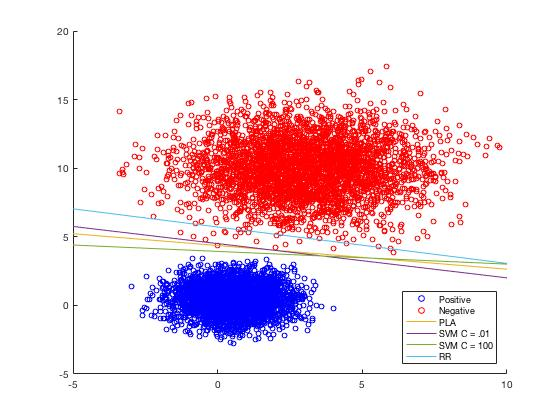
\includegraphics[width=\linewidth]{data.jpg}
  \caption{Training Data and Separating Hyperplanes}
\end{figure}

\newpage{}
\subsubsection{Implementation}
\begin{verbatim}
%
% Trains algorithms and plots hyperplanes
%
function empirical_observations(Xtest, Xtrain, ytest, ytrain)
    % Split training data into classes
    [d, m] = size(ytrain);
    pos = [];
    neg = [];
    
    for i = 1: d
        if ytrain(i) == 1
            pos = [pos; Xtrain(i,:)];
        else
            neg = [neg; Xtrain(i,:)];
        end
    end
    
    % Train algorithms
    [w_perceptron, w_0_perceptron] = train_perceptron(Xtrain, ytrain);
    [w_rr, w_0_rr] = train_rr(Xtrain, ytrain, 1);
    [w_svm_01, w_0_svm_01] = train_svm_primal(Xtrain, ytrain, 0.01);
    [w_svm_100, w_0_svm_100] = train_svm_primal(Xtrain, ytrain, 10000);
    
    % Test algorithms
    loss_perceptron = test_algorithm(Xtest, ytest, w_perceptron, w_0_perceptron);
    loss_rr = test_algorithm(Xtest, ytest, w_rr, w_0_rr);
    loss_svm_01 = test_algorithm(Xtest, ytest, w_svm_01, w_0_svm_01);
    loss_svm_100 = test_algorithm(Xtest, ytest, w_svm_100, w_0_svm_100);
    
    % Display empirical errors
    disp('Perceptron Loss ');
    disp(loss_perceptron);
    
    disp('Ridge Regression Loss ');
    disp(loss_rr);
    
    disp('SVM C = .01 Loss ');
    disp(loss_svm_01);
    disp('SVM C = .01 Support Vector Count ');
    disp(count_support_vectors(Xtrain, w_svm_01, w_0_svm_01));
    
    disp('SVM C = 100 Loss ');
    disp(loss_svm_100);
    disp('SVM C = 100 Support Vector Count ');
    disp(count_support_vectors(Xtrain, w_svm_100, w_0_svm_100));
    
    % Define hyperplanes
    a_p = -1 * w_perceptron(1)/w_perceptron(2);
    b_p = -1 * w_0_perceptron/w_perceptron(2);
    x_p = -5:10;
    y_p = a_p * x_p + b_p;
    
    a_rr = -1 * w_rr(1)/w_rr(2);
    b_rr = -1 * w_0_rr/w_rr(2);
    x_rr = -5:10;
    y_rr = a_rr * x_rr + b_rr;

    a_svm_01 = -1 * w_svm_01(1)/w_svm_01(2);
    b_svm_01 = -1 * w_0_svm_01/w_svm_01(2);
    x_svm_01 = -5:10;
    y_svm_01 = a_svm_01 * x_svm_01 + b_svm_01;

    a_svm_100 = -1 * w_svm_100(1)/w_svm_100(2);
    b_svm_100 = -1 * w_0_svm_100/w_svm_100(2);
    x_svm_100 = -5:10;
    y_svm_100 = a_svm_100 * x_svm_100 + b_svm_100;
    
    % Plot points
    figure,
    scatter(pos(:,1), pos(:,2), 25, 'b'),
    hold on,
    scatter(neg(:,1), neg(:,2), 25, 'r'),
    plot(x_p, y_p),
    plot(x_svm_01, y_svm_01),
    plot(x_svm_100, y_svm_100),
    plot(x_rr, y_rr),
    hold off,
    legend('Positive', 'Negative', 'PLA', 'SVM C = .01', 'SVM C = 100', 'RR', 
           'Location', 'southeast');
end

%
% Calculates the empirical risk of trained hypothesis
%
function loss = test_algorithm(X, y, w, w_0)
    [m, d] = size(X);  % Size of input matrix
    loss = 0;          % Value of loss
    
    % Sum over each training example
    for i = 1:m
        if y(i) * (dot(w, X(i, :)) + w_0) <= 0
            loss = loss + 1;
        end
    end
    
    loss = loss / m;
end

%
% Calculates the number of support vectors
%
function count = count_support_vectors(X, w, b)
    [m, d] = size(X);  % Size of input matrix
    count = 0;         % Number of support vectors
    min = 100;
    
    % Calculate the margin of each sample
    for i = 1:m
        margin = abs(dot(w, X(i, :)) + b);
        
        % Check in double precision range
        if margin <= 1.0001 && margin >= .9999
            count = count + 1;
        end
    end
end
\end{verbatim}
\end{document} 